% Options for packages loaded elsewhere
\PassOptionsToPackage{unicode}{hyperref}
\PassOptionsToPackage{hyphens}{url}
%
\documentclass[
]{article}
\usepackage{lmodern}
\usepackage{amssymb,amsmath}
\usepackage{ifxetex,ifluatex}
\ifnum 0\ifxetex 1\fi\ifluatex 1\fi=0 % if pdftex
  \usepackage[T1]{fontenc}
  \usepackage[utf8]{inputenc}
  \usepackage{textcomp} % provide euro and other symbols
\else % if luatex or xetex
  \usepackage{unicode-math}
  \defaultfontfeatures{Scale=MatchLowercase}
  \defaultfontfeatures[\rmfamily]{Ligatures=TeX,Scale=1}
\fi
% Use upquote if available, for straight quotes in verbatim environments
\IfFileExists{upquote.sty}{\usepackage{upquote}}{}
\IfFileExists{microtype.sty}{% use microtype if available
  \usepackage[]{microtype}
  \UseMicrotypeSet[protrusion]{basicmath} % disable protrusion for tt fonts
}{}
\makeatletter
\@ifundefined{KOMAClassName}{% if non-KOMA class
  \IfFileExists{parskip.sty}{%
    \usepackage{parskip}
  }{% else
    \setlength{\parindent}{0pt}
    \setlength{\parskip}{6pt plus 2pt minus 1pt}}
}{% if KOMA class
  \KOMAoptions{parskip=half}}
\makeatother
\usepackage{xcolor}
\IfFileExists{xurl.sty}{\usepackage{xurl}}{} % add URL line breaks if available
\IfFileExists{bookmark.sty}{\usepackage{bookmark}}{\usepackage{hyperref}}
\hypersetup{
  pdftitle={Demographics of Hate},
  pdfauthor={Conor McMahon},
  hidelinks,
  pdfcreator={LaTeX via pandoc}}
\urlstyle{same} % disable monospaced font for URLs
\usepackage[margin=1in]{geometry}
\usepackage{graphicx,grffile}
\makeatletter
\def\maxwidth{\ifdim\Gin@nat@width>\linewidth\linewidth\else\Gin@nat@width\fi}
\def\maxheight{\ifdim\Gin@nat@height>\textheight\textheight\else\Gin@nat@height\fi}
\makeatother
% Scale images if necessary, so that they will not overflow the page
% margins by default, and it is still possible to overwrite the defaults
% using explicit options in \includegraphics[width, height, ...]{}
\setkeys{Gin}{width=\maxwidth,height=\maxheight,keepaspectratio}
% Set default figure placement to htbp
\makeatletter
\def\fps@figure{htbp}
\makeatother
\setlength{\emergencystretch}{3em} % prevent overfull lines
\providecommand{\tightlist}{%
  \setlength{\itemsep}{0pt}\setlength{\parskip}{0pt}}
\setcounter{secnumdepth}{-\maxdimen} % remove section numbering
\usepackage{booktabs}
\usepackage{longtable}
\usepackage{array}
\usepackage{multirow}
\usepackage{wrapfig}
\usepackage{float}
\usepackage{colortbl}
\usepackage{pdflscape}
\usepackage{tabu}
\usepackage{threeparttable}
\usepackage{threeparttablex}
\usepackage[normalem]{ulem}
\usepackage{makecell}
\usepackage{xcolor}

\title{Demographics of Hate}
\author{Conor McMahon}
\date{8/31/2021}

\begin{document}
\maketitle

\begin{verbatim}
## Warning: package 'kableExtra' was built under R version 4.0.3
\end{verbatim}

This package runs some basic demographic statistics using the FBI's
annual report on hate crimes in the United States. Reports from
2017-2020 are aggregated here.

\hypertarget{data-sources}{%
\section{Data Sources}\label{data-sources}}

Hate crime rates are tracked by the FBI. The FBI figures include only
crimes which were self-reported by law enforcement departments around
the US to the FBI. All federal law enforcement groups are required to
report hate crimes, but state and local groups have variable policies.
Additionally, hate crimes are only reported if the case is tried as a
hate crime, which is likely to vary based on social context both in
terms of the region in which the crime occurred and the category
targeted by the hate attack.

\begin{itemize}
\tightlist
\item
  Hate crime reports are from a database of
  \href{https://crime-data-explorer.fr.cloud.gov/pages/home}{annual FBI
  reports}
\end{itemize}

Population statistics came from several different sources. The US Census
Bureau was used where possible, but the Census primarily tracks sex and
race/ethnicity and does not have much data on religion, gender identity,
or sexual orientation.

\begin{itemize}
\tightlist
\item
  Racial population estimates are from the US
  \href{https://www.census.gov/quickfacts/fact/table/US/PST045219}{Census}
\item
  Religious afiliation population estimates are from the
  \href{https://www.pewforum.org/religious-landscape-study}{Pew Research
  Center}
\end{itemize}

Several groups are not covered by the above resources.

\begin{itemize}
\tightlist
\item
  I took an estimate of 700,000 Sikhs in the United States from the
  \href{http://saldef.org/archive/learn-about-sikhs/\#.WaR7qyiGOM9}{Sikh
  American Legal Defense Fund}
\end{itemize}

All population estimates were taken as a single baseline, under the
assumption that the overall fraction of the country made up of each
group changed little in this 10-year tracking period. This is a BAD
ASSUMPTION for some groups, but the population data I have access to
don't support a higher-resolution analysis. I've tried to help correct
for changing population by focusing not on per-capita rates of hate
crimes but on the relative risk of crime compared to the risk
experienced by the population at large. This statistic is unaffected by
changes in population if all groups change in population in similar
ways.

In this framing, relative risk is calculated on an annual basis as how
much \emph{more or less likely} a person is to experience a hate crime
based on belonging to one of the target groups tracked by the FBI,
relative to the overall population. For example, if a group makes up 2\%
of the population but 10\% of hate crimes, members of that group are 5
times as likely to experience hate as the average person.

It's important also to keep in mind that people can be members of
multiple groups at once. The FBI tracks hate against racial and ethnic
groups, religions, gender identity and sexual orientation.

There are some groups tracked by the FBI which I was not able to find
good population statistics for and which I didn't include here. These
are:

\begin{itemize}
\tightlist
\item
  ``Anti-Other Race/Ethnicity/Ancestry''
\item
  ``Anti-Multiple Races, Group''
\item
  ``Anti-Mental Disability''
\item
  ``Multiple Bias''
\item
  ``Anti-Other Religion''
\item
  ``Anti-Physical Disability''
\item
  ``Anti-Multiple Religions, Group''
\item
  ``Anti-Other Christian''
\item
  ``Anti-Bisexual''
\item
  ``Anti-Gender Non-Conforming''
\end{itemize}

For some of these groups, like the physically and mentally disabled, I
specifically did not attempt to include estimates because definitions of
disability can vary widely and I am not an expert in those areas. I
don't want to spread misinformation regarding risk of hate based on my
own inability to judge how many people `should' be included in the
overall population.

I also have less confidence in my estimates for populations of people
based on gender identity and sexual orientation. These data are not
tracked by the US Census, and many categories have experienced large
fluctuations in recent decades not just based on changes in the actual
way people experience gender and sexuality, but because of changing
ideas about what these words themselves mean, changes in the level of
comfort people have being out, increased visibility and representation
of LGBTQ people, etc. As an example of this, the results below show a
steady increase since 2012 of violence against trans people. I think
this is likely a) an undercount of actual violence experienced by trans
people and b) an artifact of evolving ideas across police departments in
the country on what actually constitutes hate, and an increased
understanding that anti-trans violence is an actual issue, and c)
resultant from ongoing changes in how trans people think about their own
identity.

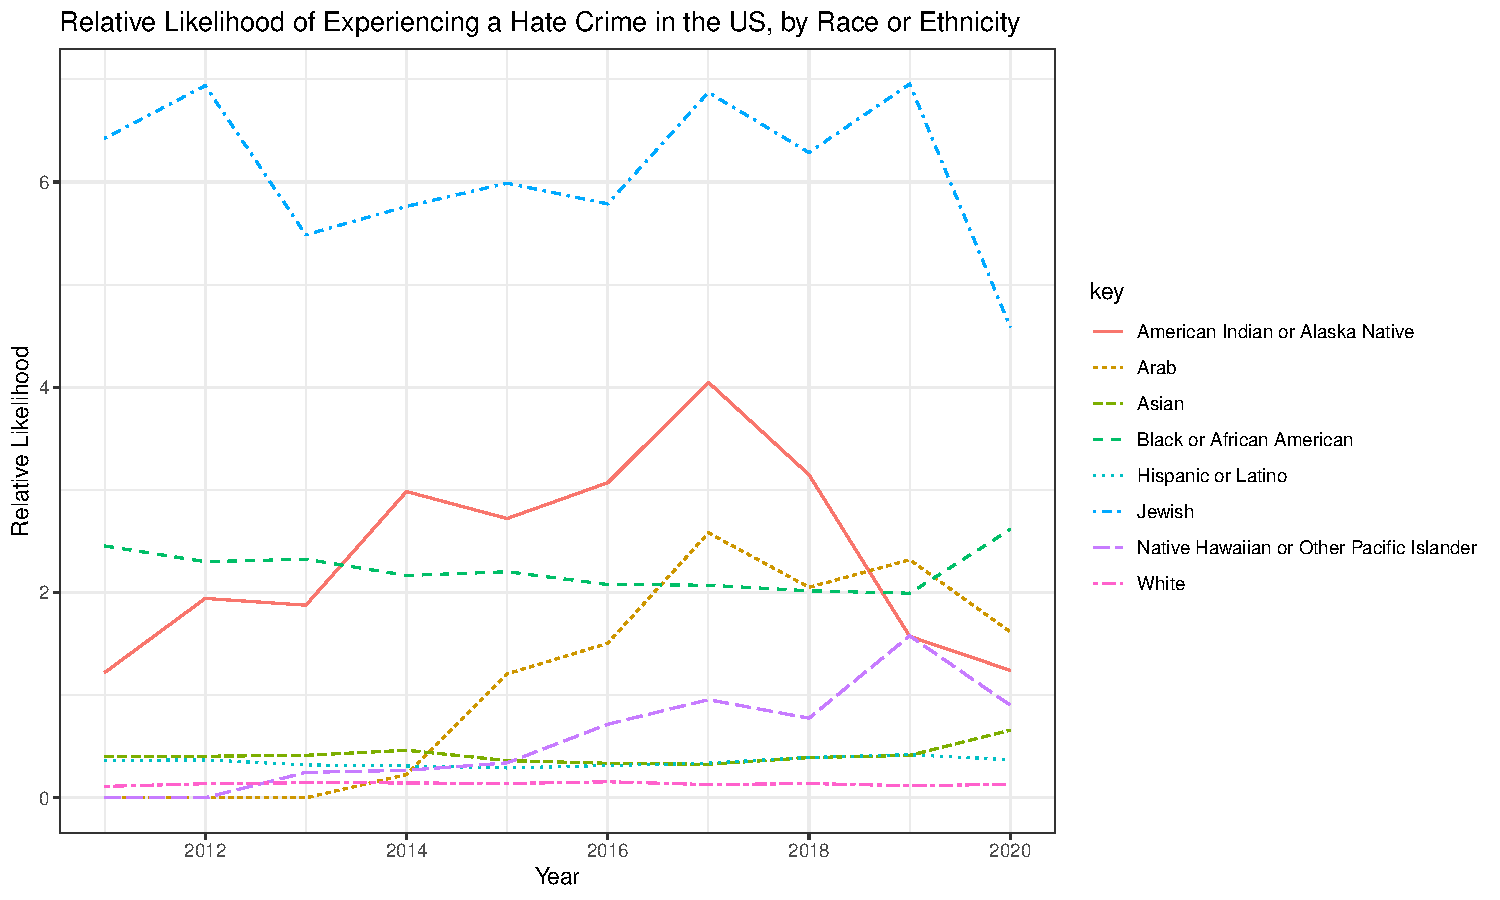
\includegraphics{demographics_of_hate_files/figure-latex/unnamed-chunk-1-1.pdf}
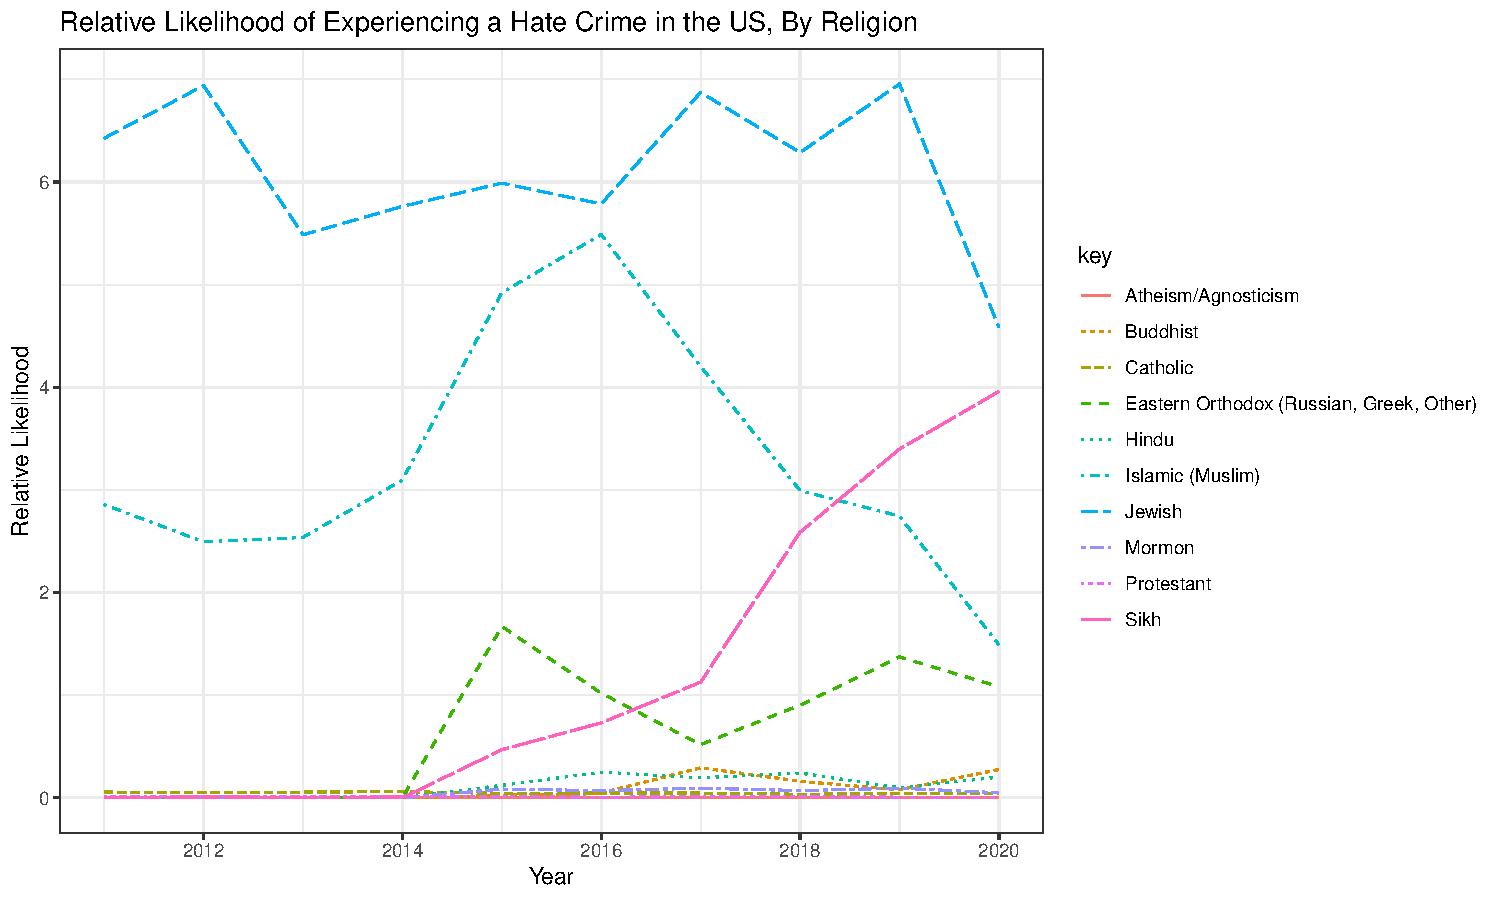
\includegraphics{demographics_of_hate_files/figure-latex/unnamed-chunk-1-2.pdf}
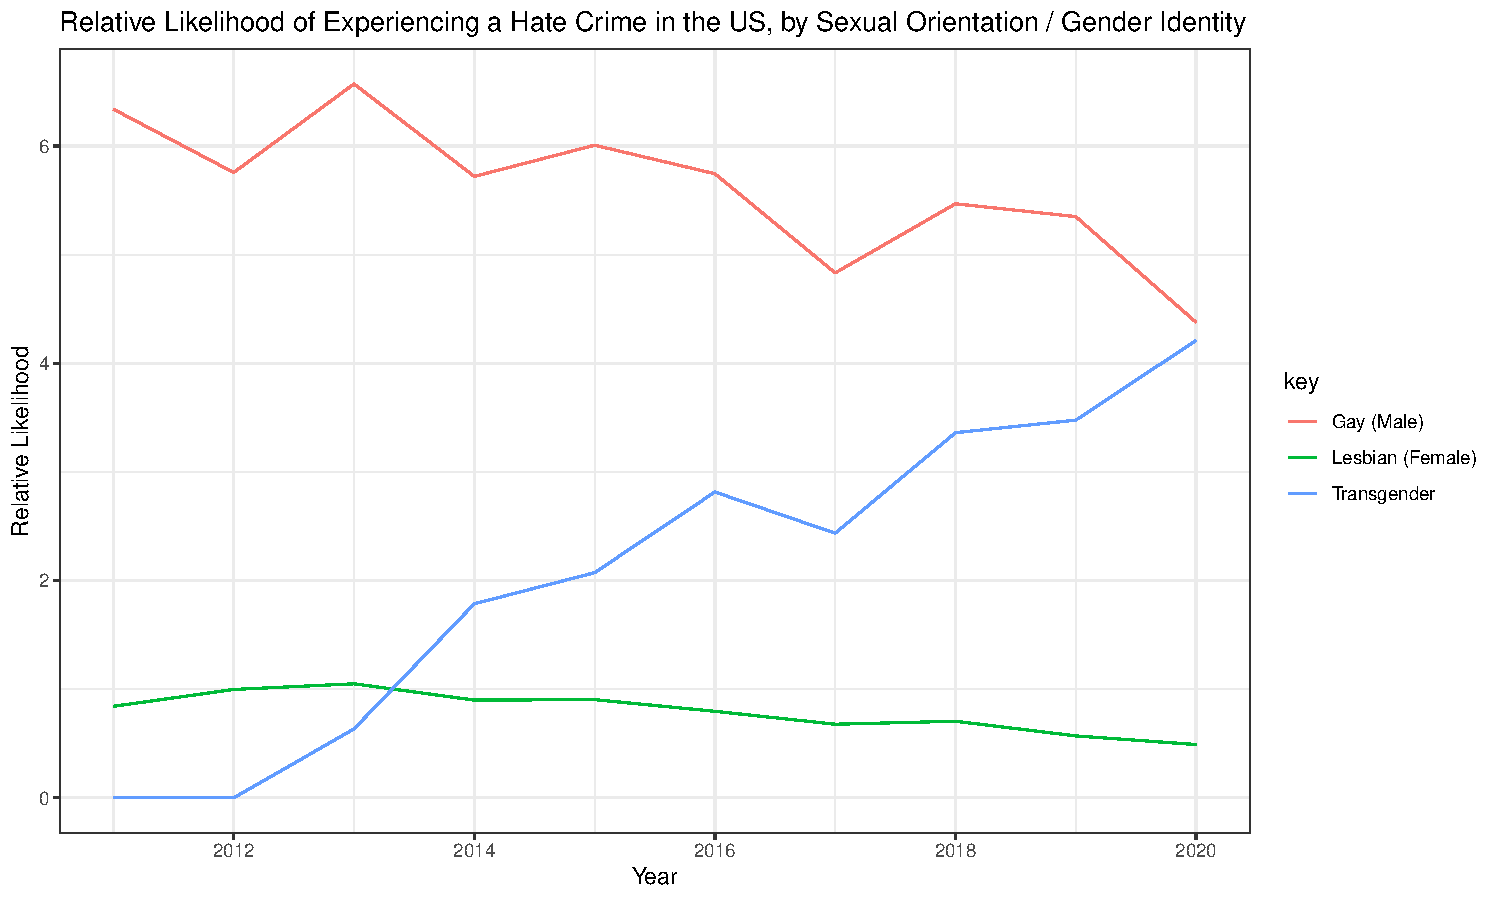
\includegraphics{demographics_of_hate_files/figure-latex/unnamed-chunk-1-3.pdf}

The above graphs show changes in relative risk fraction over the last
decade within the US, grouped by a) race or ethnicity; b) religion; c)
gender identity or sexual orientation.

Below are the same data tabulated and ordered in descending order of
relative risk rate, taken as decadal averages from the period 2011 to
2020.

\begin{table}[H]
\centering
\begin{tabular}[t]{l|r|r|r|r|r}
\hline
Demographic Group & Total Hate Crimes & Population & Crimes Per Capita & Fraction of All Crimes & Relative Risk Rate\\
\hline
Jewish & 7681 & 6099084.0 & 0.0012594 & 0.1324653 & 6.9718572\\
\hline
Gay (Male) & 7033 & 6134394.0 & 0.0011465 & 0.1212900 & 6.3469384\\
\hline
Islamic (Muslim) & 1926 & 2889040.0 & 0.0006667 & 0.0332155 & 3.6906092\\
\hline
American Indian or Alaska Native & 1286 & 2632102.0 & 0.0004886 & 0.0221781 & 2.7047902\\
\hline
Black or African American & 19968 & 43587472.0 & 0.0004581 & 0.3443649 & 2.5361108\\
\hline
Transgender & 860 & 1926026.0 & 0.0004465 & 0.0148314 & 2.4719042\\
\hline
Sikh & 195 & 700000.0 & 0.0002786 & 0.0033629 & 1.5421688\\
\hline
Arab & 444 & 1766012.0 & 0.0002514 & 0.0076572 & 1.3918251\\
\hline
Lesbian, Gay, Bisexual, or Transgender (Mixed Group) & 2852 & 14445198.0 & 0.0001974 & 0.0491851 & 1.0930030\\
\hline
Lesbian (Female) & 1339 & 8349325.0 & 0.0001604 & 0.0230922 & 0.8878192\\
\hline
Eastern Orthodox (Russian, Greek, Other) & 224 & 1605022.0 & 0.0001396 & 0.0038631 & 0.7726136\\
\hline
Native Hawaiian or Other Pacific Islander & 81 & 642008.8 & 0.0001262 & 0.0013969 & 0.6984565\\
\hline
Asian & 1492 & 17186320.0 & 0.0000868 & 0.0257308 & 0.4805972\\
\hline
Hispanic or Latino & 4103 & 56510571.0 & 0.0000726 & 0.0707597 & 0.4019455\\
\hline
White & 6708 & 240991029.0 & 0.0000278 & 0.1156851 & 0.1540946\\
\hline
Hindu & 54 & 2247031.0 & 0.0000240 & 0.0009313 & 0.1330393\\
\hline
Buddhist & 45 & 2247031.0 & 0.0000200 & 0.0007761 & 0.1108661\\
\hline
Jehovahs Witness & 30 & 2568035.0 & 0.0000117 & 0.0005174 & 0.0646719\\
\hline
Mormon & 51 & 5136071.0 & 0.0000099 & 0.0008795 & 0.0549711\\
\hline
Catholic & 656 & 66768917.0 & 0.0000098 & 0.0113133 & 0.0543907\\
\hline
Protestant & 314 & 149588054.0 & 0.0000021 & 0.0054152 & 0.0116206\\
\hline
Female & 270 & 163712248.0 & 0.0000016 & 0.0046564 & 0.0091302\\
\hline
Atheism/Agnosticism & 64 & 73189005.0 & 0.0000009 & 0.0011037 & 0.0048409\\
\hline
Male & 112 & 157292159.0 & 0.0000007 & 0.0019315 & 0.0039419\\
\hline
Heterosexual & 197 & 306559209.0 & 0.0000006 & 0.0033974 & 0.0035575\\
\hline
\end{tabular}
\end{table}

\end{document}
